\documentclass{article}
\usepackage[utf8]{inputenc}
\usepackage[ruled,linesnumbered]{algorithm2e}
\usepackage{fullpage}
\usepackage{amsthm}
\usepackage{cancel}
\usepackage{hyperref}
\usepackage{graphicx}

\newtheorem{lemma}{Lemma}
\newtheorem{theorem}{Theorem}
\newtheorem{definition}{Definition}

\newcommand{\A}{\mathcal{A}}

\title{Asynchronous Converge}
\author{Vinesh Sridhar}
\date{}

\begin{document}

\maketitle

\section{What We Did Last Semester}
\begin{itemize}
 \item 9/2 ``How do I present a paper" + definitions of pki, real/ideal world, etc.
 \item 9/8 Outline the ParallelBroadcast protocol
 \item 9/15 MPC and VRFs; how does Fmine work?
 \item 9/17 Lemma Diagrams: Correctness and Complexity
 \item 9/22 What makes a good research question?
 \item 9/24 Julian suggested that ACS is a rough analog to PBC; what is ACS?
 \item 9/29 Bracha RBC; ACS Case Study: HoneyBadgerBFT
 \item 10/2 Why does Bracha RBC need 'Ready' messages?; ACS Case Study: Dumbo 1 and 2
 \item 10/13 What are the upshots of the combinatorial lemmas (5, 9, 6, 10)?
 \item 10/15 Lifting from Dumbo2: PRBC + Converge?
 \item 10/21 Not PRBC + Converge because the communication of PRBC is too high. Begin studying the converge problem in more detail
 \item 10/22 What is the Converge Problem? Is it properly defined (Jon thinks not)?
 \item 10/27 Define the game that the adversary plays each round by allowing/delaying messages.
 \item 10/30 Focus on the honest parties in the game; pigeonhole stuff; eminent parties; what will an inductive proof look like?
 \item 11/3 Can't prove anything about an arbitrary m---what can we prove? Jon's inductive random variable: Pi,j,k: the probability party i receives mj by round k--can we guarantee that this consistently decreases in certain situations?
 \item 11/10 v-eminent parties, heavy parties, push/pull/push \& pull; 
 \item 11/12 we tried to plug the v-eminence formula into wolfram alpha
 \item 11/17 how do we ground our discussion of v-eminence; consider fixing n or consider the case where n is arbitrary; consider the random variable Yi,r, the number of honest parties' inputs pi has recieved after round r \& Xi,r, the number of honest parties who have received mi after r rounds
 \item 11/19 Do we want each HP to end up with all messages from any n - 2t HPs or do we want each HP to end up with all messages from a certain subset of the HPs?
 \item 12/1 What is the adversary's best strategy? Matrix formulation to track the probability a given HP does not have a given message.
 \item 12/3 Jansen's lemma to show that the party wants to ``spread out" the bundles evenly? Markov chains? What happens as we follow a few rounds of this matrix stuff?
\end{itemize}

\section{PBC Lemmas in Brief}
\subsection{Complexity}
\begin{itemize}
\item Theorem 6: PBC has complexity $\tilde O(n^2k^4)$
\item Lemma 11: $|distinct(M)| = 2n$
\item Theorem 4: Distinct Converge Random is t-secure and has complexity $O(nlogn * |distinct(M)| * m * s)$
\item Theorem 3: Converge random is t-secure and has complexity $O(nlogn * |M| * m * s)$
\item Lemma 9: Extension of Lemma 5; after a round p of converge, $>= min\{2^p, h_p\}$ honest parties will receive some initial honest message with overwhelming probability. $h_p$ is the number of remaining HPs in round p.
\item Lemma 7: Propagate has complexity $O(|M| * m * s)$ ($m$ is probability param, $s$ is message length)
\item Lemma 6: During propagate, An honest party p sends at most $2 * |M| * m/n$ messages to any party q with overwhelming probability. 
\item Lemma 5: In AddRandomEdgesAdaptive (models Converge's message propagation for 1 subround), after a round the number of HPs and that have seen some initial honest message will double with overwhelming probability, even with an adaptive adversary
\end{itemize}

\subsection{Correctness}
\begin{itemize}
\item Theorem 5: PBC is $t$-secure
\item Lemma 13: PBC is $t$-valid (b/c of the initial multicast by honest senders)
\item Lemma 12: PBC is $t$-consistent
\item Lemma 10: Each $(b_i, s_i)$-committee contains $>= 1$ HP and $<= R$ corrupted parties with overwhelming probability. $R$ is the number of rounds in the protocol.
\item Lemma 8: Propagate is the real-world equivalent of $F_{prop}$.
\end{itemize}



\section{The Converge Problem}
\subsection{Definition}
As described by Tsimos et al.~\cite{PBC}, in the converge problem each honest party begins with a set of messages. We wish to guarantee that, by the end of the converge protocol, every honest party holds a superset of the union of the initial honest messages. The authors consider a synchronous setting with an adaptive adversary. Put another way, we want every honest party $p$ to hold a set $S_p$ by the end of the converge protocol such that:
\begin{center}
    $S_p \supseteq \bigcup\limits_{p \in \mathcal H} M_p$ 
\end{center}

\subsection{Asynchronous Converge}
If we were to move this to an asynchronous setting, what would change? By the nature of asynchronous protocols in which the adversary controls the network, honest parties cannot wait to receive messages from all other parties because a corrupted party may choose to not send anything. It is only safe for honest parties to wait for $n - t$ messages every round. Furthermore, because honest parties does not know which parties are honest or corrupted, they cannot distinguish between an honest sender whose message is being delayed and a corrupted sender who will not sent anything. Therefore, it is inevitable that not all honest messages may be delivered or agreed upon by all honest parties, meaning that we must relax the definition of the converge problem. If in each round, honest parties wait for $n - t$ messages, that means that at least $n - 2t$ are honest. This suggests two natural definitions for asynchronous converge:
\begin{enumerate}
    \item There exists some $\mathcal H^* \subset \mathcal H$, $|\mathcal H^*| \geq n-2t$ such that for all $p \in \mathcal H$, $S_p \supseteq \bigcup\limits_{p \in \mathcal H^*} M_p$ 
    \item For all $p \in \mathcal H$, there exists some $\mathcal H^* \subset \mathcal H$, $|\mathcal H^*| \geq n-2t$ such that $S_p \supseteq \bigcup\limits_{p \in \mathcal H^*} M_p$ 
\end{enumerate}

Clearly the first is a stronger than the second because the honest parties actually agree on a subset of the honest parties whose messages they receive. Perhaps this is the only useful one--the protocol is called converge, after all.

Note that this definition bears resemblance to the problem known as Asynchronous Common Subset, in which honest parties must agree on a subset of the input messages and must ensure that a significant portion of that subset are honest messages.

\section{AddRandomEdgesAdaptive}

\emph{AddRandomEdgesAdaptive} is the model that Tsimos et al. \cite{PBC} use to prove how fast messages propagate in parallel broadcast despite the presence of an active adversary. The algorithm represents a round of the converge protocol and focuses on the spread of a single message. Parties are represented as vertices in a graph. Let $S$ be the set of honest parties, $\mathcal H$, that hold some message $m$ at the beginning of the round. First, we take a party $p$ in $S$ and attempt to draw an edge from $p$ to all other vertices, each with some probability $q$. Parties multicast their bundles in the synchronous protocol, so every other party is guaranteed to receive $m$ with probability $q$. We repeat this for every party in $S$. Now the adversary can choose which parties to corrupt. It has partial information---it can only see edges that are incident to corrupted parties. 

They prove that, for every choice of parties the adversary could corrupt in this round, there is an overwhelming probability that the set of honest parties that hold $m$ after the corruptions take place is at least $2|S|$. This is what is shown in lemma 5.

\subsection{Adapting AddRandomEdgesAdaptive to the Asynchronous Case}
To make this model fit our case, we could add this step: Before we generate the edges, the adversary can iterate through all vertices and select the $n - t$ parties from which they can receive bundles from. In the next step, if the adversary has allowed it, we add an edge from $p \in S$ to some other party $v$ with probability $q$. Otherwise, the probability an edge is drawn from $p$ to $v$ is 0.

The only problem with this is that the model only focuses on one message at a time. But when we are arguing about how the adversary allocates bundles, that applies to all messages.

\section{Asynchronous Common Subset}
The term Asynchronous Common Subset (ACS) appears to have been first used by Miller et al.~\cite{miller2016honey}. They describe a protocol in which $n$ parties each submit an arbitrary message (e.g. an encrypted batch of transactions). Each party outputs a subset of those messages, and the protocol guarantees that every honest party will agree on some subset $S$ and that $|S| \geq n - t$. This protocol is used as a building block for their BFT atomic broadcast protocol, HoneyBadgerBFT. Every epoch, each party inputs a batch of transactions into an ACS execution. Honest parties sort the result in some canonical way and output it as a block.

The authors took inspiration from two sources. The first is an atomic broadcast protocol proposed by Cachin et al. \cite{cachin2001secure}. Here, each party $p_i$ first waits to receive $n - t$ messages. $p_i$ compiles this into a set $W_i$ and inputs it into multi-valued validated Byzantine agreement. MVBA checks the validity of each $W_i$ and outputs a single, valid set. As above, parties sort this set in some canonical order, and output it to their logs. Miller et al. state that this protocol reduces ACS to MVBA because the end result is the same, an agreed-upon subset of at least $n - t$ messages. However, the communication complexity of MVBA is high for large messages, leading the authors to look to a protocol developed by Ben-Or et al. \cite{ben1994asynchronous}. In their paper, Ben-Or et al. present this protocol:

\begin{algorithm}\label{ben-or-prot}
\caption{Ben-Or et al. Agreement on a Common Subset \cite{ben1994asynchronous}}

\SetKwProg{Throughout}{throughout}{:}{}
\SetKwProg{Define}{define}{:}{}
\SetKwProg{Upon}{upon}{:}{}
\SetKwProg{On}{upon}{:}{}
\SetKwProg{When}{when}{:}{}
\SetKwProg{Init}{initialize}{:}{}
\SetKwProg{Main}{main}{:}{}
\SetKwProg{Meanwhile}{meanwhile}{:}{}
\SetKwProg{At}{at}{:}{}
\SetKwProg{cWhile}{while}{:}{}
\SetKwProg{Procedure}{procedure}{:}{}

\SetKw{Trigger}{trigger}

Let $Q$ be a function that assigns a binary value to each party. $Q$ is dynamic---not all parties need to be assigned a value at the same time.\\
Code for player $P_i$:\\
1. For each $P_j$ for whom you know that $Q(j) = 1$, participate in BA$_j$ with input 1.\\
2. Upon completing $2t+1$ ($n - t$ if $n = 3t + 1$) BA protocols with output 1, enter input 0 to all BA protocols for which you haven't entered a value yet.\\
3. Upon completing all $n$ BA protocols, let you $SubSet_i$ be the set of all indices $j$ for which BA$_j$ had output 1. Output $SubSet_i$.

\SetAlgoLined
\SetAlgoNoEnd
\end{algorithm}

Miller et al. suggest that, by the totality property of reliable broadcast, if some honest party $P_i$ outputs a message in RBC$_j$, then we can say that $P_i$ knows that $Q(j) = 1$. Ben-Or et al. show that $SubSet_i$ is shared among all honest parties and has size at least $n - t$. Therefore, ACS can be constructed with reliable broadcast and asynchronous binary Byzantine agreement.

\subsection{Properties}
\begin{enumerate}
    \item Consistency: All honest parties output the same subset of input messages.
    \item Set quality: At least $n - 2t$ messages sent by honest parties get into the final output. This means that at least half of the final output is honest.
    \item Termination: Honest parties can only wait for at most $n - t$ input messages.
\end{enumerate}
 
\subsection{Case Studies}
\subsubsection{HoneyBadgerBFT}
This is the algorithm the authors present. Note the similarities to the algorithm by Ben-Or et al. shown above.

\begin{algorithm}\label{honeybadger-acs}
\caption{Asynchronous Common Subset  from Miller et al. \cite{miller2016honey}}

For party $P_i$ with message $v_i$: \\
Input $v_i$ to RBC$_i$ as the sender.\\
Upon outputting $v_j$ from RBC$_j$, input 1 to BA$_j$ if not done already.\\
Upon outputting 1 from $n - t$ BA instances, input 0 to each BA $P_i$ has not yet provided input to.\\
Wait for all BA instances to complete. Let $C \subset [1...n]$ be the indexes of each BA for which $P_i$ outputted 1. Wait for each $v_j$ from RBC$_j$ for each $j \in C$. Output the resulting set of messages.
\SetAlgoLined
\SetAlgoNoEnd
\end{algorithm}
For $P_i$ to output 1 in BA$_j$, some honest party $P_k$ must have input 1 to BA$_j$, meaning that $P_k$ must have output some message $v_j$ in RBC$_j$. By totality of RBC, all honest parties will eventually receive $v_j$. This, combined with the fact that ABA is guaranteed to terminate after all parties input their bits and RBC is guaranteed to terminate if the sender is honest, means that this ACS implementation must terminate. If honest party $P_i$ outputs 1 in BA$_j$, all honest parties output 1 in BA$_j$, guaranteeing consistency. And by definition, at least $n - t - t = n - 2t$ messages come from honest parties, guaranteeing set quality.

They claim that the communication complexity of their RBC implementation (a modification of Bracha RBC) is $O(n|v| + \lambda n^2\log n)$ and the communication complexity of ABA is $O(\lambda n)$ per node, where $\lambda$ is the security parameter and $|v|$ is the message size. The total complexity is $O(n^2|v| + \lambda n^3\log n)$, dominated by the $n$ RBCs. What communication complexity does not reveal, however, is that, because parties must output some $v_j$ from RBC$_j$ before contributing to BA$_j$ most of the time, Asynchronous Byzantine Agreement is the real bottleneck of the protocol. Guo et al. considered this problem when they designed their Dumbo BFT protocols \cite{guo2020dumbo}.
\subsubsection{Dumbo1 and 2}
Because the runtime of HoneyBadgerBFT's ACS protocol depends on how long the $n$ ABAs take, Guo et al. aimed to construct an ACS protocol that required fewer instances of ABA. Their first attempt resulted in Dumbo1, in which parties elects a committee of $\kappa$ (independent of $n$) parties after the initial RBCs. Committee members, 1 of which is honest with overwhelming probability, then wait to receive $n - t$ messages from the initial RBCs. Once they receive those messages, committee member $p_i$ encodes them as a list $S_i$, where $S_i[j] = 1$ if $p_i$ output some $v_j$ from RBC$_j$.

The committee members then perform an ``index RBC", in which they share their $S_i$'s (much smaller in size than the original messages). Then $\kappa$ ABAs occur, where some party $p_k$ inputs 1 to ABA$_i$ if upon receiving all of the corresponding messages indicated in $S_i$. Once a party outputs 1, then it will input 0 into all of the remaining ABAs that it has not yet offered input to. Once all the ABAs finish, every honest party will wait for all the messages specified in any $S_i$ such that they output 1 in ABA$_i$.

If an honest party outputs 1 in ABA$_i$, then it must have received all of the messages indicated in $S_i$. By totality of the initial RBCs, all honest parties will eventually receive all of the messages indicated in $S_i$. With overwhelming probability, some committee member $p_h$ is honest, so $S_h$ contains messages that eventually reach all honest parties. $S_h$ is of size at least $n - t$, so the output must contain at least $n - 2t$ honest messages. Therefore, this protocol guarantees termination, consistency, and set quality.

As in HoneyBadgerBFT's ACS protocol, Dumbo1's ACS protocol is separated into two phases: the sending phase, in which the initial RBCs disseminate each party's message and the agreement phase, in which the index RBCs and ABAs occur. In both protocols, the agreement phase's purpose is to settle on a set of at least $n - t$ parties whose messages each honest party is guaranteed to receive if they wait long enough (by totality of the initial RBCs).


Unlike HoneyBadgerBFT, in which ABA$_i$ corresponds to a single message $v_i$, parties vote on a group of $n  - t$ messages, so only a single ABA needs to output 1 for the parties to be able to return. However, in Dumbo1 parties still need to wait for all $\kappa$ ABAs to finish before they can output (just in case another ABA evaluates to 1). In addition, the ABAs are still entangled with the RBCs: in order to vote in ABA$_i$, parties must wait to receive $S_i$ and the $n - t$ messages it corresponds to (or until some other ABA terminates). In Dumbo2, the authors deal with both of these issues by adding a threshold signature scheme to RBC and by replacing the ABAs with MVBA.

As Miller et al. observed, Chachin et al.'s MVBA implementation is inefficient because each party inputs $n - t$ messages in their entirety to the protocol \cite{miller2016honey} \cite{cachin2001secure}. Guo et al. circumvents this in Dumbo2 by agreeing upon a proxy for the messages rather than the messages themselves \cite{guo2020dumbo}. This proxy takes the form of a signature $\sigma_i$. If $\sigma_i$ is valid, that means that some honest party must have received $v_i$ from RBC$_i$. Its size depends on the security parameter and so is much smaller than the messages size. A proof $\sigma_i$ requires $t + 1$ signature shares so it is valid only if some honest party has contributed a share. By totality of RBC, if $\sigma_i$ is valid, every honest party will eventually receive $p_i$'s message. Therefore, parties can trust that, if they see a valid proof, they will receive the corresponding message.

This allows us to shift the agreement phase's predicate from the receipt of $n - t$ messages (as in Dumbo1) to the receipt of $n - t$ valid proofs. In Dumbo1, to vote, parties would have to wait for messages before they voted on an index set in their corresponding ABA. In Dumbo2, the proofs are self-contained, so the predicate can be evaluated immediately. This means that all information required for the MVBA can be front-loaded, as opposed to the information required for the $\kappa$ ABAs in Dumbo1, which depend on receiving messages or receiving the output of one of the ABAs. 
\subsection{ACS through the Converge Problem}

As described above, ACS has two phases, the sending phase and the agreement phase. Converge guarantees that parties end up with a shared core-set of messages, but each party is not aware what the core-set is, only that it is a subset of the messages they hold. 

So converge can roughly perform the sending phase, but without the safeguard of totality that RBC provides. We need a way of culling the messages: how about ``not-proofs". We could use a similar threshold signature scheme as Dumbo2. After converge, parties distribute a signature share for messages they \emph{do not} have. $t + 1$ signature shares form a not-proof $\cancel \sigma_i$. This won't work because it may happen that $< t + 1$ honest parties are missing $m_i$, and so they may not be able to form the signature.

What if each party used RBC to share the indices of the messages they do not have? RBC is guaranteed to terminate for honest parties, but we can only wait for $n - t$ to finish. A corrupted party might end up sharing a list that causes honest parties to discard a member of the core-set.

It may be the case that all but 1 honest party has some message $m$ (is this true?). How would that single honest party tell the rest not to output $m$? It seems that a converge-like protocol is too weak to do this. The adversary could just block that party from sending anything.




\section{The Game}
Something about each subround of converge. The adversary chooses which messages to deliver. n - t in total, n - 2t honest, t corrupt. Include a picture.
\subsection{The Game II: Narrowed Down to Honest Parties}
Bipartite thingy

\subsection{Definitions}
\subsubsection{v-eminent parties}
\subsubsection{heavy parties}
\subsection{What's the Adversary's Best Strategy?}
\subsubsection{Matrix of Probabilites}
\subsubsection{Markov Chains IDK?}

\section{Lemma 5 Rewrite}

This lemma fixes a message $m$ and examines a single round, where $S$ is the set of honest parties that send a bundle containing $m$ this round. $H$ is the set of honest parties and $V$ is the set of all parties. We model this using the algorithm AddRandomEdgesAdaptive. All parties in $S$ send a bundle to every party, in which $m$ is included with probability $q$. This is modeled by drawing an edge from each vertex in $S$ to a vertex in $V$ with probability $q$. After that is done, the adversary can examine the edges that point to corrupted nodes and choose to corrupt any nodes it wants, revealing more edges along the way. It can corrupt at most $t$ nodes over all rounds.

We want to show that, if $|S|$ is at most half of $n - t$ (even if $\mathcal A$ has yet to corrupt $t$ parties), the number of honest parties that hold $m$, even after the adversary corrupts parties at the end of that round, is still $\geq 2|S|$ with high probability. 

Let $Y_u$ be a binomial random variable such that $Y_u = 1$ iff $u \in H$ has nonzero degree in $G$.\\
\textbf{Lemma 5.} \textit{Let $(G, H') \leftarrow AddRandomEdgesAdaptive_\mathcal A(V, S, H, m)$. Fix $\epsilon \in (0, 1)$. Let $|S| \leq \epsilon * n / 2$ (where $\epsilon * n = n - t$ ). We will show that
\begin{center}
    $\Pr\big [\sum_{u \in H'} Y_u \geq 2|S|\big ] \geq 1 - p$,
\end{center}
where $p = max\{n * e^{-\epsilon *k/5}, (\frac{e}{2})^{-\epsilon *k/2}\}$} ($k$ is $\Theta(\kappa)$, the security parameter).

\begin{proof}
First, we define $E_{H'}$ as the event that AddRandomEdgesAdaptive outputs $(\cdot, H')$. Let $E_{H^*}$ be the ``worst'' of such events, i.e.
\begin{center}
    $\Pr \big[\sum_{u \in H'} Y_u \geq 2|S| \big | E_H'\big ] \geq \Pr\big [\sum_{u \in H^*} Y_u \geq 2|S| \big | E_{H^*}\big ]$
\end{center}
for all possible $E_{H'}$. Now we split our analysis into two cases: one in which $|S| \leq \epsilon * n/5$ and the other in which $|S| > \epsilon * n/5$.\\
\textit{Case 1: $|S| \leq \epsilon * n/5$}

In this case, we lower bound $\Pr\big [\sum_{u \in H^*} Y_u \geq 2|S| \big | E_{H^*}\big ]$ by applying a lower tail Chernoff bound. To do that, we need to show that $\{Y_u\}_{u\in H^*}$ are independent. Of course, this must be true because edges to any $u$ in $H^*$ are generated uniformly and independently, and so they are independent when conditioned on $E_{H^*}$ as well. We will apply the bound to the random variable $Y = \sum_{u \in H^*}Y_u$.
\begin{center}
    $\mu = E[Y|E_{H^*}] = \sum_{u \in H^*} \Pr\big [Y_u = 1 \big | E_{H^*}\big ] \geq |H^*| * (1 - (1 - k/n)^{|S|}) \geq \epsilon * n * (1 - (1 - k/n)^{|S|})$\\
    $\geq \epsilon * n * (1 - (1 - k/n)^1) = \epsilon * k$. 
\end{center}
Plugging $\delta = 1/2$ into the Chernoff bound, we get
\begin{center}
    $\Pr\big [Y < \mu / 2 \big | E_{H^*}\big ] < (\frac{e^{-1/2}}{(1/2)^{1/2}}) ^{\epsilon * k} = (\frac{e}{2})^{-\epsilon*k/2}$
\end{center}

We are looking for the probability $\Pr[Y \geq 2|S| | E_{H^*}] = 1 - \Pr\big [Y < 2|S| \big | E_{H^*}\big ]$ and so we must show that $\mu \geq 4|S|$ for $\Pr\big [Y < 2|S| \big | E_{H^*}\big ] < \Pr\big [Y < \mu / 2 \big | E_{H^*}\big ]$ to be true. We show that if $k$ is chosen carefully, this is the case:

\begin{center}
    $\mu \geq \epsilon * n * (1 - (1 - k/n)^{|S|})$\\
    $\mu \geq \epsilon * n * (1 - e^{-k|S|/n})$ as $1 + (-k/n) \leq e^{-k/n}$\\
    $\mu \geq 5 * |S| * (1 - e^{-k*\epsilon / 5})$ as $|S| \leq \epsilon * n / 5$ and so $\epsilon * n \geq 5 * |S|$\\
    $\mu \geq 4 * |S|$ if we set $k \geq 10/\epsilon$
\end{center}

Therefore, for $|S| < \epsilon * n / 5$, 
\begin{center}
    $\Pr \big [Y \geq 2|S| \big | E_{H'} \big]$ \\
    $ \geq \Pr\big [Y \geq 2|S| \big | E_{H^*}\big ]$ \\ $ = 1 - \Pr\big [Y < 2|S| \big | E_{H^*}] $ \\ $> 1 - \Pr\big [Y < \mu / 2 \big | E_{H^*}\big ]$ \\ $ > 1 - (\frac{e}{2})^{-\epsilon*k/2}$
\end{center}

for any $H'$ that results from AddRandomEdgesAdaptive.\\
\textit{Case 2: $|S| > \epsilon * n/5$}\\
Here there are a relatively large amount of senders, so we lower bound $\Pr\big [\sum_{u \in {H^*}} Y_u \geq 2|S| \big | E_{H^*}\big ]$ by computing $\Pr\big [(\sum_{u \in {H^*}} Y_u) = |H^*| \big | E_{H^*}\big ]$. We know that $H^* \geq \epsilon * n$ and we assumed at the start that $|S| \leq \epsilon * n / 2$, so $H^* > 2*|S|$. Therefore,
\begin{center}
    $\Pr\big [\sum_{u \in {H^*}} Y_u \geq 2|S| \big | E_{H^*}\big ] \geq \Pr\big [(\sum_{u \in {H^*}} Y_u) = |H^*| \big | E_{H^*}\big ]$,
\end{center}
so it suffices to lower bound $\Pr\big [(\sum_{u \in {H^*}} Y_u) = |H^*| \big | E_{H^*}\big ]$, the probability that all parties in $H^*$ have $m$ by the end of the round. 

\begin{center}
$\Pr\big [(\sum_{u \in {H^*}} Y_u) = |H^*| \big | E_{H^*}\big ] $\\ $= \Pr\big [(\bigcap_{u \in {H^*}} Y_u = 1)\big | E_{H^*}\big ]$ \\$ = 1 - \Pr\big[(\bigcup_{u \in {H^*}} Y_u = 0)\big | E_{H^*}\big ]$ \\ $\geq 1 - \sum_{u \in {H^*}} \Pr\big [Y_u = 0 \big | E_{H^*}\big ]$

\end{center}

If we assume that, in the worst case, all $u \in H^*$ start the round without $m$, then for all $u \in H^*$, $\Pr[Y_u = 0 | E_{H^*}] = (1 - k/n)^{|S|} < (1 - k/n)^{\epsilon * n/5} \leq e^{-\epsilon * k / 5}$, where $k/n$ is the probability an edge is drawn from a party in $S$ to some other party in $V$, so  $1 - \sum_{u \in {H^*}} \Pr[Y_u = 0 | E_{H^*}] = 1 - |H^*| * (e^{-\epsilon * k / 5}) \geq 1 - n * e^{-\epsilon * k / 5}$, as $|H^*| \leq n$. We have shown that, for $ \epsilon * n/5 < |S| \leq \epsilon * n / 2$, 
\begin{center}
    $\Pr\big [\sum_{u \in {H'}} Y_u \geq 2|S| \big | E_{H'}\big ] \geq \Pr\big [\sum_{u \in {H^*}} Y_u \geq 2|S| \big | E_{H^*}\big ] \geq 1 - n * e^{-\epsilon * k / 5}$
\end{center}
for any $H'$ that results from AddRandomEdgesAdaptive.


\end{proof}

Tsimos et al \cite{PBC} explain that Lemma 5 ``[states] that during the propagation process, an adversary corrupting a party that just sent does not get any further information about who to corrupt next". That's not entirely true. The assumptions we've made proclude the adversary from learning certain information about the honest parties, but they still learn something from the currently corrupted parties, like which parties in $S$ may have $m$. Lemma 5 shows that the adversary, with high probability, cannot do anything with this information to significantly decrease message propagation.

The only other lemma that discusses the propagation properties of converge, lemma 9, considers the propagation of the protocol over multiple rounds. It considers two cases, $|S_\rho| \leq \epsilon * n / 2$ and $|S_\rho| > \epsilon * n / 2$, where $S_\rho$ is the set of senders in round $\rho$ and $\epsilon * n = n - t$. In the first case, the authors apply lemma 5 inductively, to show that the number of parties that have some message doubles each round. In the second case, because there are many senders, they show that the probability that at least one honest party in that round does not receive the message is negligible. That means that no matter what parties the adversary corrupts at the end of that round, all honest parties will have the message. Once again, the proof focuses on a single message and not a group of messages. 

They suggest that the reason that ParallelBroadcast is secure under an active adversary whereas RandomBroadcast (their single-sender BC that uses gossiping) is only secure under an active adversary is because of the nature of converge, which is used for PBC but not for RandomBroadcast. I interpreted the claim as the authors implying that, due to the sheer amount of messages being sent back and forth through converge, it was hard for the adversary to choose which parties to corrupt. But it seems like the real defense against an active adversary is just the speed at which messages spread through converge, not necessarily the structure of the protocol. I suspect that converge could have been used in RandomBroadcast to make it adaptively secure, but then the complexity would be too high for a single-sender broadcast protocol (In RBC parties only gossip if they have received a message for the first time whereas in PBC/converge, they gossip everything they have every round).


\section{Protocol sketches}

Rather than changing the recipients at each round of converge, we have randomly selected a fixed number of them at the beginning, encoded as gossip vectors. $g_{i \rightarrow j}[k] = 1$ indicates that $P_i$ has selected $P_j$ to be in its gossip vectors for message $m_k$. We want these gossip relations to be bidirectional, so each $P_i$ sends $g_{i \leftarrow j}$ to $P_j$. This way if $P_i$ has chosen to send $m_k$ to $P_j$ once it has received it, $P_j$ will send $P_i$ $m_k$ upon receiving. Because we are in an asynchronous setting, however, an honest party is only able to receive $n - t$ gossip vectors from distinct parties, so each honest party is paired with at most $n - t$ parties, at least $n - 2t$ of which are honest. 

We must show that there is a set of messages $M_\mathcal H$ of messages from honest parties such that (1) $|M_\mathcal H| \geq n-2t$ and (2) each honest party $P_i$ delivers a set of messages $M_i \supseteq M_\mathcal H$ by the end of the protocol. Note that we base the security properties of this protocol off of those in Murmur, which requires totality and validity in the case of the sender. We do not require consistency, which is why parties deliver as soon as they receive a new message that has a valid signature.

We can represent these gossip relationships in $n - t$ separate graphs, one for each $p \in \mathcal H$. Consider the graph $G_k$ for $P_k$: the vertices in the graphs are the honest parties, and an edge exists between two parties if they have a \emph{gossip relation with respect to $m_k$}. E.g. $P_i$ and $P_j$ have a gossip relation with respect to $m_k$ if $g_{i \rightarrow j}[k] = 1$ and $P_j$ received $g_{i \rightarrow j}$ or $g_{j \rightarrow i}[k] = 1$ and $P_i$ received $g_{j \rightarrow i}$, meaning that if either receives $m_k$, they will send it to the other in the subsequent round.

To show that $P_i$ delivers a set of messages $M_i \supseteq M_\mathcal H$, we must show that our gossip vectors are large enough such that $n - 2t$ of the graphs $G_i$ are connected. We also must prove that no information about the structure of these graphs is leaked to $\mathcal A$---this requires that the protocol be divided into rounds to accommodate the ``cross-traffic" that obscures correspondence. Therefore, another problem is that we may run out of rounds before some honest party receives enough messages.

(Note: we assume private channels, i.e., $\mathcal{A}$ sees that a message
is sent from $P_i$ to $P_j$ but does not learn the message's contents.)

\begin{algorithm}\label{prot:1}
\caption{Parallel Murmur 1 (from the perspective of $P_i$ with input $m_i$)}

\SetKwProg{Throughout}{throughout}{:}{}
\SetKwProg{Define}{define}{:}{}
\SetKwProg{Upon}{upon}{:}{}
\SetKwProg{On}{upon}{:}{}
\SetKwProg{When}{when}{:}{}
\SetKwProg{Init}{initialize}{:}{}
\SetKwProg{Main}{main}{:}{}
\SetKwProg{Meanwhile}{meanwhile}{:}{}
\SetKwProg{At}{at}{:}{}
\SetKwProg{cWhile}{while}{:}{}
\SetKwProg{Procedure}{procedure}{:}{}

\SetKw{Trigger}{trigger}

\SetAlgoLined
\SetAlgoNoEnd

\On{initialization}{
    sample gossip vectors $g_{i\rightarrow 1},\dots,g_{i\rightarrow n}$ for each $P_j$ ($g_{i\rightarrow j}[k] = 1$ if $P_j$ is in $P_i$'s gossip set for $m_k$ and 0 otherwise)\;
    \For{$j = 1$ to $n$}{
        send $g_{i\rightarrow j}$ to $P_j$\;
    }
    
    Let $delivered$ be an $n$-length vector all initialized to $\bot$\;
    Let $delivered[i] \leftarrow m_i$\;
}
\On{receiving gossip vector $g_{j\rightarrow i}$ from $P_j$}{
    \For{$k = 1$ to $n$}{
        \If{$g_{j\rightarrow i}[k] = 1$}{
            $g_{i \rightarrow j}[k] \leftarrow 1$\;
        }
    }
}


\On{receiving $n-t$ gossip vectors}{
    \Trigger distribute
}

\Procedure{distribute}{
    \For{$r = 1$ to $R$}{
        \Trigger sendBundles($r$)\;
        wait until $n - t$ round-$r$ bundles have been received\;
        \If{$P_i$ receives some $m_k$ such that $delivered[k] = \bot$ and $m_k$ is valid}{
            $delivered[k] \leftarrow m_k$
        }
    }

}

\Procedure{sendBundles(r)}{
    \For{$j = 1$ to $n$}{
        Initialize list $L_j$\;
        \For{$k = 1$ to $n$}{
            
            \If{$g_{i\rightarrow j}[k] = 1$}{
                append $(delivered[k], k)$ to $L_i$
            }
            
            \Else{
                append $(-, k)$ to $L_i$
            }
        }
    }
    
    Pad and encrypt each $L_j$ to form a bundle $B_{j,r}$\;
    Send $B_{j,r}$ to $P_j$\;
}

\end{algorithm}

The following definition is based on the (single-sender) probabilistic broadcast protocol of \url{https://arxiv.org/pdf/1908.01738.pdf}.

\begin{definition}
A \emph{parallel probabilistic broadcast} protocol has the following properties:
\begin{itemize}
    \item No duplication: for each $i$, each party delivers at most one $m_i$
    \item Integrity: if a party delivers $m_i$, and $P_i$ is honest, then 
        $P_i$ input $m_i$
    \item $\epsilon$-Output intersection: with probability
    at least $(1-\epsilon)$, there is a set $M^*\subseteq M_H$ of size
    at least $n-2t$ such that for all honest $P_i$, 
    the set of messages $M_i$ delivered by $P_i$
    satisfies $M^*\subseteq M_i$ (where $M_H$ is the set of honest parties' inputs)
\end{itemize}
\end{definition}

What do we expect $\epsilon$ to depend on?
\begin{itemize}
    \item number of parties
    \item (maximum) number of corrupted parties
    \item number of rounds
    \item distribution of gossip vectors
\end{itemize}

\section{The Game III: $\mathcal{A}$ the plumber}
We came up with this game to demonstrate how the independence of the rounds in our original conception of converge, adapted from parallel broadcast, allows us to analyze it in a more straightforward way. As before, each round is represented by a bipartite graph of parties on both sides. However, we now introduce the concept of \emph{pipes}. Pipes are connections between two parties $p_i$ and $p_j$ with respect to a given message $m_k$. For example, if in round $r$, $p_i$ has an $m_k$-\emph{pipe} to $p_j$, then if $p_i$ has $m_k$ by the beginning of round $r$, it will send it to $p_j$ in its bundle. Whether that bundle is delivered is still determined by the adversary. An $m_k$-pipe is created from party $p_i$ to $p_j$ in round $r$ with some probability $p$ that matches the probability that $p_i$ would include $m_k$ in its bundle to $p_j$ in round $r$ if it has it. 

Because a message is included in a bundle with an independent, random probability, it does not matter whether the pipes are generated before execution or at the time a bundle is being populated. Thus, in our game we can generate a graph of pipes for the whole execution at the beginning. We get the benefit of a definitive sender and receiver that we wanted when exploring gossip vectors without having to deal with delivering gossip subscribes in an asynchronous setting.

\subsection{The Game}

\begin{enumerate}
    \setcounter{enumi}{-1}
    \item Instantiate the graph $G$. 
    \begin{enumerate}
        \item For rounds $1$ to $R$ create a set of $n$ nodes in $G$
        \item For every node $p_{i,r}$ for $1 \leq r < R$ in $G$, do the following:
        \begin{enumerate}
            \item For every message $m_k$ and party $p_j$, draw an $m_k-$pipe from $p_{i,r}$ to $p_{j,r+1}$
        \end{enumerate}
    \end{enumerate}
    
    \item Let an \emph{edge} from $p_{i,r}$ to $p_{j,r+1}$ be the set of all pipes $C$ between those two nodes in $G$. The adversary can choose to add an edge which will establish all the pipes in $C$. If $p_j$ is honest, the adversary can add the edge as long as the in-degree of $p_{j,r+1}$ is $\leq n-t$. 
    
    \item Repeat the previous step until the in-degree of every node $p_{i, r}$, where $p_i$ is honest and $1 < r \leq R$, is $n-t$.
    
\end{enumerate}

The goal of our protocol is for there to be some $\mathcal H^* \subseteq \mathcal H$ such that $|\mathcal H^*| \geq n - 2t$ and every honest party outputs a set of messages $M_i \supseteq M_{\mathcal H^*}$. In the game, party $p_i$ receives a message $m_k$ if there is a path of established $m_k$-pipes from any $p_{k, \_}$ to $p_{i, \_}$ node. Thus, the adversary wins if there exists an honest party $p_i$ such that for all $\mathcal H^*$, there is a $p_j$ such that no path of $p_j$-pipes exists from any $p_{j, \_}$ to $p_{i, \_}$.

We make some assumptions about what the adversary can do in the game. It can only add $n-t$ edges that point to some honest $p_{j, r}$. And the way the pipes work implies that if an honest party receives a message for some later round, it will wait until it advances to that round to process it. Is this realistic? We argue that a few modifications to the protocol will accomplish this. 


\subsection{The Corresponding Protocol}

\begin{algorithm}\label{prot:1}
\caption{Asynchronous Converge 1 (from the perspective of $P_i$ with input $m_i$)}

\SetKwProg{Throughout}{throughout}{:}{}
\SetKwProg{Define}{define}{:}{}
\SetKwProg{Upon}{upon}{:}{}
\SetKwProg{On}{upon}{:}{}
\SetKwProg{When}{when}{:}{}
\SetKwProg{Init}{initialize}{:}{}
\SetKwProg{Main}{main}{:}{}
\SetKwProg{Meanwhile}{meanwhile}{:}{}
\SetKwProg{At}{at}{:}{}
\SetKwProg{cWhile}{while}{:}{}
\SetKwProg{Procedure}{procedure}{:}{}

\SetKw{Trigger}{trigger}

\SetAlgoLined
\SetAlgoNoEnd

\On{initialization}{
    Let $delivered$ be an $n$-length vector all initialized to $\bot$\;
    Let $delivered[i] \leftarrow m_i$\;
    \Trigger distribute
}

\Procedure{distribute}{

    \For{$r = 1$ to $R$}{
        \Trigger sendBundles($r$)\;
        wait until $n - t$ round-$r$ bundles have been received\;
        
        \For{each bundle $B_{i, r'}$ received during this round}{
            
            $Let$
            \If{$r' = r$ and $P_i$ receives some $m_k$ such that $delivered[k] = \bot$ and $m_k$ is valid}{
                $delivered[k] \leftarrow m_k$
            }
            
            \uElseIf{$r' < r$}{
                discard $B$
            }
            
            \uElseIf{$r' > r$}{
                buffer $B$ until iteration $B.round$
            }
        }
    }
}

\Procedure{sendBundles(r)}{

    \For{$j = 1$ to $n$}{
        Initialize list $L_j$\;
        \For{$k = 1$ to $n$}{
            Let $c$ be the outcome of a weighted coinflip with probability $p$.
            \If{$c = 1$}{
                append $(delivered[k], k)$ to $L_i$
            }
            
            \Else{
                append $(-, k)$ to $L_i$
            }
        }
    }
    
    Pad and encrypt each $L_j$ to form a bundle $B_{j,r}$\;
    Send $B_{j,r}$ to $P_j$\;
}

\end{algorithm}

The three if conditions in $sendBundles$ make the protocol line up with the game. Honest parties discarding bundles from round $r$ are once they receive $n - t$ round-$r$ bundles corresponds to the game preventing the adversary from increasing the in-degree of honest nodes above $n - t$. Buffering bundles from later rounds means that bundles are always processed in round-order, which corresponds with the piping system we introduce. Consequently,
a party $P_i$ in an execution of the protocol
outputs a message $m_j$ if and only if there is a directed path from $v_{j,0}$
to $v_{i,R}$.

\subsection{Bounds on the Adversary's Probability of Winning}
As a first attempt, we will bound the probability that the adversary wins
a simplified version of the game, in which
all pipes are shown to the adversary at the start of the game.
(It's possible the adversary wins this game with probability 1, in which case
we might want to see if we can prove something about a lower threshold than $n-2t$,
e.g., a bound on the probability that $|\mathcal H^*|\geq1$.)
This will lay the foundation for analyzing a more realistic game, in which
the adversary must make decisions using limited information about the probability
that a round $r$ bundle from $P_i$ to $P_j$ contains a particular message $m_k$.

\subsection{How Powerful is the Adversary?}
The intuition of our gossip protocol is that, if the adversary cannot read the contents of bundles and can block only so many bundles from being delivered, after a sufficient number of rounds, messages have propagated enough such that the adversary cannot win, no matter what it does. This level of partial knowledge is hard to specify and analyze, so we have come up with several simplified scenarios that will allow us to step up to a full analysis if necessary. We specify four different adversaries:
\begin{itemize}
    \item $\mathcal A_1$: The adversary has full knowledge of all generated pipe graphs at the beginning of the protocol. This is known as the \emph{offline}, \emph{full-information} adversary
    \item $\mathcal A_2$: The adversary has full knowledge of all generated pipe graphs up to the current round. This is known as the \emph{online}, \emph{full-information} adversary.
    \item $\mathcal A_3$: The adversary has partial knowledge of all generated pipe graphs up to the current round. This is known as the \emph{online}, \emph{partial-information} adversary and is closest to the actual adversary in our setting.
    \item $\mathcal A_4$: The adversary chooses which bundles to deliver randomly.
\end{itemize}

Each adversary's probability of winning should satisfy this inequality:
\begin{center}
    $Pr[\mathcal A_1$ wins $] \geq Pr[\mathcal A_2$ wins $] \geq Pr[\mathcal A_3$ wins $] \geq Pr[\mathcal A_4$ wins $]$ 
\end{center}

Therefore, if $Pr[\mathcal A_1$ wins $]$ is sufficiently low, we don't need to do any more analysis.

\subsection{Considering $\mathcal A_1$}
As described above, $\mathcal A_1$ knows the contents of all pipe graphs at the beginning of execution. Therefore, it knows what messages will be contained in any bundle it decides to deliver. Therefore, given each uniformly-generated pipe graph, is there a PPT algorithm that can determine whether the adversary can win? And if so, what is a winning bundle-delivery schedule?
\subsubsection{Notation}
Let $G_i$ represent $p_i$'s pipe graph. It is a $R$-round bipartite graph and its edges are uniformly chosen. 
Let $G^*$ encode the adversary's bundle-delivery schedule. An honest party $p_i$ delivers its message to all other parties iff in $G^* \cap G_i$, there is a path from $p_i$ in round 1 to all other honest parties in round $R$. 
\subsubsection{Flow?}
A natural strategy is to reduce this scenario into a problem concerning $n$ distinct flow networks. If the adversary runs a max flow algorithm on $G^* \cup G_i'$, where $G_i'$ is $G_i$ with a sink node connected to round-$R$ vertices with edges that have capacities = 1, then the max flow of the configuration exactly equals the number of honest parties that will receive $m_i$. 

This suggests the generic algorithm template presented in Algorithm~\ref{prot:2}: 

\begin{algorithm}\label{prot:2}
\caption{$\mathcal A_1$ max-flow generic strategy}

\SetKwProg{Throughout}{throughout}{:}{}
\SetKwProg{Define}{define}{:}{}
\SetKwProg{Upon}{upon}{:}{}
\SetKwProg{On}{upon}{:}{}
\SetKwProg{When}{when}{:}{}
\SetKwProg{Init}{initialize}{:}{}
\SetKwProg{Main}{main}{:}{}
\SetKwProg{Meanwhile}{meanwhile}{:}{}
\SetKwProg{At}{at}{:}{}
\SetKwProg{cWhile}{while}{:}{}
\SetKwProg{Procedure}{procedure}{:}{}

\SetKw{Trigger}{trigger}

Let $G^*$ be a full round graph.\\
\While{$G^*$ does not satisfy the constraints of the game}{
    \For{all $e \in G^*$}{
        compute $goodness(e)$
    }
    pick the best $e$ to remove
    $G^* \leftarrow G^* - e$
}

\SetAlgoLined
\SetAlgoNoEnd
\end{algorithm}

\section{Special case: probability of sending = 1}

Consider the special case where each party includes all messages they've received in each bundle.

Define $S_i^r$ to be the set of parties that have $m_i$ at the beginning of round $r$. What does $S^r_i$ tell us about $S^{r+1}_i$?

As a small example, let $n=4$ (so $t=1,$ $n-t=3$, $n-2t=t+1=2$).

High-level idea: want to show that for all rounds, either:
\begin{enumerate}
    \item $\forall i,j$ s.t. $i\neq j$, $|\overline{R_i}\cup R_j|\geq 1$ (everyone learns something new next round), or
    \item $\exists$ set of $n-2t$ honest parties $C$ s.t. $|\bigcap_{i\in C} R_i|\geq k_{\cap}$ (there is a relatively large set of honest parties who share a core set)
\end{enumerate}

\begin{lemma}[Jon's lemma, $n=4$ case]
Suppose there are $4$ parties, of which 3 are honest. 
At the end of round 1 (i.e., once
each honest party has received at least $n-2t$ messages from other
honest parties), one of the following holds:
\begin{enumerate}
    \item $\forall P_i,P_j$ s.t. $i\neq j$, $P_i$ has some message that $P_j$ does not, or
    \item there exist two parties that hold the same two messages.
\end{enumerate}
\end{lemma}
\begin{proof}

\end{proof}

\begin{lemma}[Jon's lemma, general case]
Suppose there are $n$ parties, of which $t$ are corrupted and $n-t$ are honest. 
At the end of round 1 (i.e., once
each honest party has received at least $n-2t$ messages from other
honest parties), one of the following holds:
\begin{enumerate}
    \item $\forall$ honest $P_i,P_j$ s.t. $i\neq j$, $P_i$ has some message that $P_j$ does not, or
    \item there exist $n-2t$ honest parties that hold the same $n-2t$ messages.
\end{enumerate}
\end{lemma}

Let $D_r \subseteq \mathcal H$ be the set of honest parties such that for every $p_i \in D_r$, $\mathcal A$ delivers $p_i$'s bundle to at least $n - 2t$ distinct honest parties in round $r$.
\begin{lemma}
$\forall r, |D_r| \geq 1$.
\end{lemma}
\begin{proof}
Assume the opposite. In each round, every party must receive at least $n - 2t$ honest messages. That means that the adversary delivers at least $(n-t)(n-2t)$ honest messages. If $|D_r| = 0$, then at most $(n-t)(n-2t-1)$ messages were delivered. This is less than $(n-t)(n-2t)$, which is a contradiction.
\end{proof}

\begin{lemma}
Let $S$ be a subset of the honest messages. If $n-2t$ honest parties hold $S$ in round $r$, then all honest parties hold $S$ in round $r+1$.
\end{lemma}
\begin{proof}
Either an honest party holds all the messages in $S$ in round $r$ or they do not. If they do, then trivially they will still hold $S$ in round $r+1$. If they do not, when they receive bundles from $n - 2t$ honest parties in round $r$, at least one of those bundles will contain $S$. This must be true by quorum intersection (i.e., because any two sets of $n-2t$ honest parties must overlap at one honest party). Thus, every honest party will hold $S$ by round $r+1$.
\end{proof}

\begin{theorem}
For any $n, t$, it will take at most 4 rounds to agree on a core-set.
\end{theorem}

\begin{proof}
In round 2, every party holds $n - 2t$ messages. $|D_2| \geq 1$, so some bundle from an honest party $p_i$ is delivered to at least $n - 2t$ honest parties in round 2. Call this bundle $S$. $n - 2t$ distinct honest parties hold $S$ in round 3, so by the above lemma, all honest parties will have $S$ at the beginning of round 4. $|S| \geq n - 2t$ and $S$ is held by all honest parties, so it is a core-set.
\end{proof}

\subsection{Canetti ACS}
In Ran Canetti's PhD thesis \cite{canetti1996studies}, he proposes an interesting ACS implementation. Like the implementations we have seen in section 5, the protocol begins with an asynchronous broadcast primitive, and ACS is used to agree upon a set of $n - t$ messages to output. Unlike Ben-Or ACS \cite{ben1994asynchronous}, before running the ABAs, Canetti's ACS runs a protocol very similar to ours: for $\log n$ asynchronous rounds, parties share `index sets' that indicate what messages they have. Once a party retrieves the messages that correspond to $n - t$ index sets, they advance a round. This is basically converge in the $p=1$ case. Canetti proves that, at the end of the $\log n$ rounds, every honest party holds the same set of $n - t$ messages (though they may hold more, hence the subsequent Byzantine Agreements that select what the honest parties output). This appears to not be needed--Ben-Or et al. overcome this problem by having parties wait for messages to arrive before inputting data into each $BA$ \cite{ben1994asynchronous}. Interestingly, the idea of front-loading message-collection appears again in Dumbo2-ACS (in the form of proofs, to reduce communication complexity) \cite{guo2020dumbo}. Regardless, the proof of correctness is interesting (despite the fact that we've shown that it only takes $4$ rounds, not $\log n$ rounds, to converge). I've reproduced it (with slight modification for clarity) below:

\begin{lemma}
By the end of round $r$, every set of at most $2^r$ uncorrupted parties $D$ satisfies $|\cap_{j \in D} U_j^r| \geq m$.
\end{lemma}

\begin{proof}
The base of induction $(r=0)$ is immediate from Step 1 of the protocol (in this step, each party waits for $n-t$ messages). For the induction step, consider a set $D$ of up to $2^r$ uncorrupted parties. We first observe that for every two parties $P_j,P_k \in D$, we have $|F_j^r \cap F_k^r| \geq t + 1$ ($F_j^r$ is the set of parties from which $P_j$ has received a message by the end of round $r$), since $n \geq 3t +1$ and $|F_j^r| \geq n - t$ for each $j$. therefore, there exists at least one \emph{uncorrupted} party $P_l \in F_j^r \cap F_k^r$; e call $P_l$ an \emph{arbiter} of $P_j$ and $P_k$. part $P_j$ (resp. $P_k$) has received the $(r, S_l)$ message; furthermore, $U^{r-1}_l \subseteq S_l$. this, $U_l^{r-1} \subseteq U_j^r$ (resp. $U_l^{r-1} \subseteq U_k^r$).

Consider an arbitrary partition of the set $D$ to pairs of parties, choose an arbiter for each pair, and let $D'$ be the set of these arbiters; thus, $|D'| \leq 2^{r-1}|$. By the induction hypothesis, we have $n - t \leq |\cap_{j\in D'} U_j^{r-1}|$. Every party in $D$ has an arbiter in $D'$, thus $\cap_{j \in D'} U_j^{r-1} \subseteq \cap_j \in D U_j^r$. Therefore, we have that $n - t \leq |\cap_{j\in D} U_j^{r}|$.

Thus, at the end of $\log n$ rounds, all honest parties share $n - t$ messages.
\end{proof}



\section{General case: probability of sending = $p$}

Things to try proving:
\begin{enumerate}
    \item  Regardless of $\A$'s strategy, if at least $n-2t$ honest parties hold a core set, then the expected number of rounds until all honest parties hold a core set is at most $\rho$. (Alternative version:
    If at least $n-2t$ honest parties hold a core set, then w.h.p. all honest parties hold a core set after $\rho'$ rounds)
    \item Regardless of $\A$'s strategy, for each honest party $P_i$, the expected number of rounds until $P_i$ has received at least $n-2t$ distinct messages is at most $\sigma$.
    \item Regardless of $\A$'s strategy, for each honest party $P_i$ and each round $r$, if $P_i$ has not yet received at least $n-2t$ messages, then in the next round $P_i$ learns a new message with probability at least $\tau$.
    \item Regardless of $\A$'s strategy, for each round in which there is not yet a core set held by all parties, the expected number of honest parties who learn a new message is at least $\zeta$.
\end{enumerate}

Define a ``proto-core set'' to be a set of at least $n-2t$ messages held by at least $n-2t$ honest parties. This intuitively seems to be a tipping point.
    
Question: Suppose each honest party holds $n-2t$ distinct messages. What is the expected number of rounds until a proto-core set exists?

Let the probability of including a message in a bundle be $p < 1$.
\begin{lemma}
If $p_i$ has $< n - 2t$ messages at the start of round $r$, it learns something new during round $r$ with probability at least $p$.
\end{lemma}
\begin{proof}
Assume the opposite. During round $r$, $p_i$ receives $n - 2t$ bundles. Call the set of senders $P_{send}$. If it learns something new with probability $< p$ in round $r$, then $p_i$ must already have every message held by every $p_j \in P_{send}$. Each party starts out with a distinct message, and $|P_{send}| \geq n - 2t$, so $p_i$ must have at least $n -2t$ messages, which is a contradiction. There must be some message that some $p_j \in P_{send}$ has that $p_i$ does not. $p_i$ will receive that message with probability at least $p$.
\end{proof}
\begin{lemma}
If $p_i$ has $c < n - 2t$ messages at the start of round $r$, it learns something new during round $r$ with probability at least $1 - (1 - p)^{n - 2t - c}$.
\end{lemma}
\begin{proof}
During round $r$, $p_i$ receives $n - 2t$ bundles. Call the set of senders $P_{send}$. Call the set of messages each party in $P_{send}$ currently holds $M_{send}^\cup$. $|M^U_{send}| \geq n - 2t$, so $p_i$ could potentially learn $|M^U_{send}| - c \geq n - 2t - c$ messages. The probability it learns none of these is at most $(1 - p)^{n - 2t - c}$, so the probability it learns something is at least $1 - (1 - p)^{n - 2t - c}$.
\end{proof}

\begin{lemma}
Let $S_j$ be the set of messages $p_j$ has. Assume $p_j$ sends a bundle to $p_i$ If $p_i$ has $v < |S_j|$ messages from $S_j$, then we expect it to receive $(|S_j| - v) * p$ messages from $S_j$ in this round.
\end{lemma}

\begin{lemma}
(this is not true). Let $S_1$, $S_2$, and $S_3$ be sets of messages s.t. $|S_i| \geq n - 2t$. 1 of the 3 must share $n - 2t$ elements with the union of the other two. i.e. $|S_i \cap (S_j \cup S_k)| \geq n - 2t$ for distinct $1 \leq i, j, k \leq 3$.
\end{lemma}

Any two sets of messages that are at least size $n - 2t$ share at least 1 message, i.e. if a party receives bundles from those respective parties, they'll get two ``votes" for that message. What about 3 sets? How many messages get 2 votes in that case? Messages in the set $(S_1 \cap S_2) \cup (S_1 \cap S_3) \cup (S_2 \cap S_3)$ get at least 2 votes. How big is this set? By definition, $|S_i \cap S_j| \geq 1$, so it's at least 1. 

\begin{lemma}
If $|S_1|, |S_2|, |S_3| \geq n - 2t$, then $|(S_1 \cap S_2) \cup (S_1 \cap S_3) \cup (S_2 \cap S_3)| \geq max\{v, n - 2t - (v - 1)\}$ where $v = min\{|S_1 \cup S_2|, |S_1 \cup S_3|, |S_2 \cup S_3|\}$ if $v < (n - 2t + 1) / 2$ and  $v = max\{|S_1 \cup S_2|, |S_1 \cup S_3|, |S_2 \cup S_3|\}$ otherwise
\end{lemma}

\begin{proof}
Consider an arbitrary $S_1$ and $S_2$. We will construct an $S_3$ that minimizes $|(S_1 \cap S_2) \cup (S_1 \cap S_3) \cup (S_2 \cap S_3)|$. First let $v = |S_1 \cap S_2|$. Then $|S_1 \cup S_2| = n - 2t + n - 2t - v = n - t + 1 - v = n - t - (v - 1)$. In addition, $H \ (S_1 \cup S_2) = n - t - (n - t - (v - 1)) = v - 1$.

So if we want to minimize $|(S_1 \cap S_2) \cup (S_1 \cap S_3) \cup (S_2 \cap S_3)|$, we begin by giving $S_3$ all $v - 1$ messages held by neither $S_1$ nor $S_2$. That leaves $n - 2t - (v - 1)$ messages we have left to allocate. This gives us two cases:

\emph{Case 1 $n - 2t - (v-1) < v$:}

Then we give $S_3$ $n - 2t - (v-1)$ messages of the $v$ already shared between $S_1$ and $S_2$. Because those messages already have 2 votes, they count for nothing. Thus, only $v$ messages have at least 2 votes, so $|(S_1 \cap S_2) \cup (S_1 \cap S_3) \cup (S_2 \cap S_3)| \geq v$.

Note that as $v$ increases, the number of messages that have 2 votes increases, so $v = max\{|S_1 \cup S_2|, |S_1 \cup S_3|, |S_2 \cup S_3|\}$

\emph{Case 2 $n - 2t - (v-1) \geq v$:}

Then we give $S_3$ all $v$ messages shared between $S_1$ and $S_2$ and $n - 2t - (v-1) - v$ more. The remaining $n - 2t - (v-1) - v$ messages are held by either $S_1$ or $S_2$ but not both, so the number of messages that have two votes is $n - 2t - (v - 1) - v + v = n - 2t - (v-1) \leq |(S_1 \cap S_2) \cup (S_1 \cap S_3) \cup (S_2 \cap S_3)|$

Note that as $v$ increases, the number of messages that have 2 votes decreases, so $v = min\{|S_1 \cup S_2|, |S_1 \cup S_3|, |S_2 \cup S_3|\}$

\end{proof}

The following lemma is interesting, but probably not useful:

\begin{lemma}
Assume that all honest parties hold $n-2t$ honest messages. There must be at least $c$ messages that are held by $n - 2t - c + 1$ parties
\end{lemma}

\begin{proof}
Assume instead that $c - 1$ messages are held by $n - 2t - c + 1$ parties, and that the remaining honest messages are held by at most $n - 2t - c$ parties. If we show that the total number of messages held is less than $(n - 2t)*(n - t)$, then we have shown that at least one honest party holds less than $n - 2t$ honest messages. 

Regardless of configuration, the largest amount of messages that can be held is $(n - t) * (c-1) + (n - 2t - c) * (n - t - (c-1))$--$c$ messages are held by all $n - t$ parties and the remaining $n -t - c$ messages are held by exactly $n - 2t - c$ parties. \\
$= c(n - t)  -  (n - t) + (n - 2t)(n - t) - c(n - t) - c(n - 2t) + n - 2t + c(c-1)$\\
$= (n - 2t)(n - t) - c(n - 2t) + c^2 - t$\\
$< (n - 2t)(n - t)$ as $c \leq n - 2t$.

We have shown that, regardless of how the messages are allocated to the parties, if fewer than $c$ messages are each held by at least $n - 2t - c + 1$ parties, at least one party must have fewer than $n - 2t$ messages, contradicting our initial assumption.
\end{proof}

\subsection{Eminent Leaders}
Every round must have an eminent party. Let us call the eminent party in round $r$ $p_e^r$. This party is guaranteed to send a message to $n - 2t$ parties during round $r+1$. During round $r+1$, every party must receive a bundle from one of the parties that received a bundle from $p_e^r$ by quorum intersection of honest parties. That means that, at the start of round $r+2$, $p_e^r$ is a grandparent of all honest parties, regardless of what the adversary does. Thus, we call $p_e^r$ an \emph{eminent leader} of round $r+2$. Parties that received $p_e^r$'s bundle directly obtained a $p$th fraction of its messages (those they did not already have) in expectation. For the remaining $ \leq t$ honest parties, a $p^2$ fraction. 

This is interesting because it is an emergent property of the protocol and the adversary cannot do anything about it. We've had a lot of trouble considering the adversary's strategy, but maybe this is a way to partially circumvent it.

Some questions this brings up: how do eminent leaders affect eminent messages? Once a message is eminent, it spreads very quickly because all parties that do not have it are guaranteed to hear from a party that does in every subsequent round. It seems natural that eminent leaders may drive eminent messages. How do eminent leaders affect subsequent eminent leaders (both $p_e^r$ and $p_e^{r+1}$ as well as $p_e^r$ and $p_e^{r+2}$)?

\subsection{Potential Discoveries}
It follows from the proof in section 12 that, in every round before a coreset is formed, there must be at least one honest party that has a nonzero chance of learning at least one new honest message. Let us call that a \emph{potential discovery}. In general, if $p_i$ receives a bundle from a sender that holds $q$ messages that $p_i$ does not have, then that party has $q$ potential discoveries from that bundle. We wish to lower bound the number of potential discoveries across all parties and across all bundles in a given round, possibly as a function of the number of eminent messages/messages in the coreset.

First, we saw that the lower bound is tight, as shown in Figure~\ref{fig:one-potential}. This can be easily generalized to arbitrary $n$ by growing the size of the $n-2t$-clique at the top, and making sure that $t-1$ parties at the bottom have all honest messages. The party that has the potential discovery then holds messages $m_1$ to $m_{n-2t-1}$ and its own message, $m_{n-2t+1}$.
\begin{figure}[h]
\centering
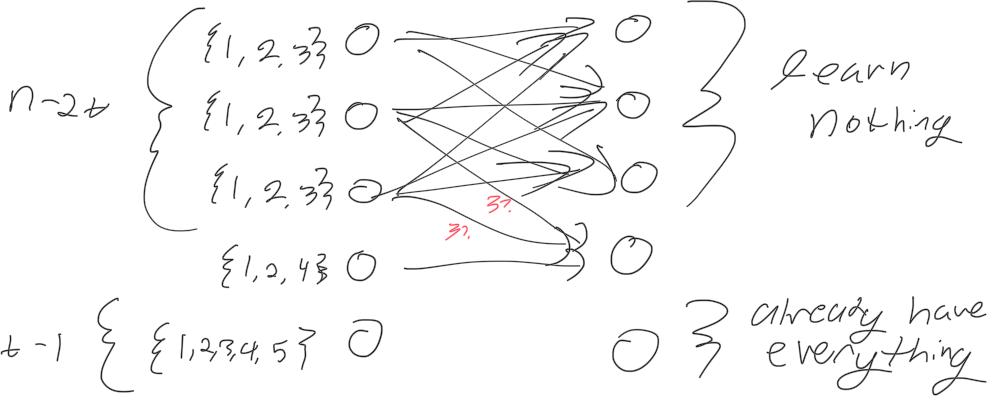
\includegraphics[scale=.4]{./figures/one-potential-discovery.png}
\caption{Showing the lower bound on the number of potential discoveries is potentially tight for $n=7, t=2$.}
\label{fig:one-potential}
\end{figure}

\subsubsection{proof sketches}

We want to show something stronger. First of all, if a message is eminent and only held by $k < n - t$ honest parties, then there must be $n - t - k$ potential discoveries for that message.

Let $c < n - 2t$ be the number of eminent messages. Intuitively, to lower-bound the number of discoveries, we ought to let each eminent message be part of a coreset, $C$, held already held by all honest parties. Every one of $p_e^r$'s, round $r$'s eminent party, messages \emph{not} in $C$ must be a potential discovery for at least one party that receives its bundle (otherwise there would be more than $c$ eminent messages). That means that, in any given round, there are at least $n - 2t - c$ potential discoveries. Of course, this does not even count the number of potential discoveries that originate from other senders. How do we incorporate these? If $c$ messages are shared amongst all honest parties, the rest are non-eminent, and have exactly $n - 2t$ messages, how does that limit what remaining messages each party can hold?

\subsubsection{Relating the number of eminent messages to the number of potential discoveries.}
In section 12, we saw that if a coreset exists, it is possible for all parties to have no potential discoveries in a round. In Figure~\ref{fig:one-potential}, we saw that if the number of eminent messages is $n - 2t$, then we can meet our lower bound: 1 potential discovery for the entire round (In which all parties but one have all of the eminent messages). What if the number of eminent messages is less than $n - 2t$? Let $c$ be the number of eminent messages.
\subsubsection{$c = n - 2t - 1$}
\begin{lemma}
If each non-eminent message is held by at most 2 parties, then each party has at least 1 potential discovery.
\end{lemma}
\begin{proof}
Assume towards a contradiction that each non-eminent message is held by at most 2 parties but some honest party $p_i$ has 0 potential discoveries. If $p_i$ has 0 potential discoveries, then it learns a new honest message with probability 0 this round. That means that $p_i$ must already hold all the messages held by the parties whose bundles were delivered to $p_i$. 

$p_i$ must receive bundles from at least $n - 2t$ honest parties. We will consider the $n - t - c$ non-eminent messages that $p_i$ has. We first note that no two parties $p_j$ and $p_k$, $j,k \neq i$ whose bundle is delivered to $p_i$ can hold the same non-eminent message $m$. If this were true, then by our assumption, $p_i$ would also hold $m$, meaning 3 parties hold $m$ at the beginning of the round, contradicting our claim. Therefore, $p_i$ holds at least $n - 2t - 1$ non-eminent messages. Furthermore, $p_i$ shares each of those non-eminent message with a distinct sender, meaning that no other honest parties can hold that message without violating our claim. $n - t - c = n - t - (n - 2t - 1) \leq n - 2t$, so only one non-eminent message can be held by the remaining $t$ parties that did not send to $p_i$. By our assumption, only two of the remaining $t$ parties can hold the last non-eminent message, so by the pigeonhole principle, some non-eminent message must be held by at least 3 honest parties, which is a contradiction. (A note on the case in which $t = 1$: if $n = 4$, then if one message is held by all parties, it is impossible for there to be $n - 2t - 1 = 1$ eminent messages. There must be 2. For $n > 4$, if $t = 1$, then there are $n - 1$ honest parties and $n - 3$ eminent messages, meaning only $2$ non-eminent messages. Parties receive $n - 2 > 2$ bundles, so by the pigeonhole principle, any party will receive two bundles from parties that share the same eminent message, meaning that, including $p_i$, 3 parties hold the message).


Note on the math: ($n - 2t + n - 2t \geq n - t + 1$, so $n - 2t - (n - 2t - 1) \geq n - t$, so $n - 2t \geq n - t - (n - 2t - 1)$)


\end{proof}

\subsection{Propagation of Eminent Messages}
A message $m_e$ is \emph{eminent} if held by at least $n - 2t$ parties ($= t+1$ if $t$ is maximal). This distinction is interesting because, upon crossing this threshold, in every subsequent round, every party that does not have $m_e$ will receive at least 1 bundle that contains $m_e$. Furthermore, if $m_e$ is held by $n - 2t - 1 + c$ parties at the start of a round, every party that does not have $m_e$ will receive at least $c$ bundles that contain $m_e$ during that round. 

Note that $1 \leq c \leq t+1$ if $m_e$ is eminent. We want to show how fast the remaining $n - t - (n - 2t - 1 + c) = t - c + 1$ (at most $t$) parties receive $m_e$. We can borrow the analysis from PBC's lemma 5 and 9~\cite{PBC}, except instead of propagating to $n$ parties, we only need to propagate to $t$ parties. 

The first lemma follows lemma 5 from PBC and shows how $c$ doubles if it is small.
\begin{lemma}
Let $\rho = m / n$ be the probability parameter, where $m = 10n/t$. If $c < t / 2$, $c$ doubles every round with high probability.
\end{lemma}
\begin{proof}
We consider two cases, one for $c \leq t/5$ and one for $c > t/5$.\\
\emph{Case 1}: \\
When $c \leq t/5$, we can apply a lower-tail Chernoff bound. Let $C$ be a random variable that tracks the size of $c$.\\
Then $E[\mu_C]$ must be at least $t * (1 - (1 - \rho)^{c})$, as there are at most $t$ parties that must receive $m_e$, and each would receive $m_e$ from at least $c$ bundles.\\
$E[\mu_C] \geq t * (1 - (1 - \rho)^{c})$\\
$\geq t * (1 - (1 - \rho))$\\
$=t * (1 - (1 - m/n))$\\
$=t * m/n$

We wish to bound $\Pr[C < \mu_C/2]$. Using a Chernoff bound, we can see that 
\begin{center}
$\Pr[C < \mu_C/2] < (\frac{e^{-1/2}}{(1/2)^{1/2}})^{\mu_C} = (\frac{e}{2})^{-\mu_C} \leq (\frac{e}{2})^{-t*m/n} \leq (\frac{e}{2})^{-10}$
\end{center}

And so $\Pr[C \geq \mu_C/2] \geq 1 - (\frac{e}{2})^{-10}$. To complete the proof, we must show that $\mu_C \geq 4c$.\\
We again start with $\mu_C \geq t * (1 - (1 - \rho)^{c})$.\\
$\geq t * (1 - e^{-\rho c})$\\
$= t * (1 - e^{-m/n *c})$\\
$\geq 5c * (1 - e^{-m/n*c})$ as $c \leq t/5$ and so $t \geq 5c$\\
$\geq 5c * (1 - e^{-m/n * (t/5)})$\\
$\geq 5c * (1 - e^{-2})$ as $m \geq 10n/t$\\
$> 4c$\\
We have shown that $\Pr[C \geq 2c] \geq 1 - (\frac{e}{2})^{-t*m/n} $.\\
\emph{Case 2}: \\
Now we will look at $t/5 < c < t/2$.

If we consider some party $p_{\cancel{m_e}}$ that does not hold $m_e$, the probability that $p_{\cancel{m_e}}$ does \emph{not} receive $m_e$ during the next round is at most $(1 - \rho)^{c}$ because at least $c$ bundles will be delivered to $p_{\cancel{m_e}}$ that contain $m_e$.\\
$(1 - \rho)^{c} < (1 - \rho)^{t/5}$ because $c > t/5$\\
$\leq e^{-\rho*t/5}$\\
$\leq e^{\frac{-m}{n} * \frac{t}{5}}$

Again let $C$ be the random variable that represents to value of $c$ after the round ends. We want to lower bound the probability that $\Pr[C \geq 2c]$.\\
$\Pr[C \geq 2c] \geq \Pr[C = t]$ because $c < t/2$ and at most $t$ parties do not know $m_e$.\\
$= 1 - \Pr[C < t]$\\
$\geq 1 - t*e^{\frac{-m}{n} * \frac{t}{5}}$.

We have shown that $c$ doubles with probability $1 - min\{(\frac{e}{2})^{\frac{-t*m}n} , t*e^{\frac{-m}{n} * \frac{t}{5}}\}$.
\end{proof}

Now we consider $c \geq t/2$, where doubling no longer makes sense. This analysis borrows from lemma 9 of PBC \cite{PBC}.
\begin{lemma}
If $c \geq t/2$ at the start of a round, then $m_e$ will be held by all honest parties by the end of the round with high probability.
\end{lemma}
\begin{proof}
During this round, every party will receive at least $t/2$ bundles that hold $m_e$, and at most $t/2$ parties do not have $m_e$ at the beginning of the round. The probability that at least one party does not have $m_e$ by the end of the round regardless is at most $(t/2) * (1 - \rho)^c$.\\
 $(t/2) * (1 - \rho)^c = (t/2) * (1 - m/n)^c$\\
 $< (t/2) * (1 - m/n)^{t/2} \leq (t/2) * e^{-\frac m n * \frac t 2}$, which is negligible in $m$.
\end{proof}

\section{A Backwards Analysis}
Any analysis of converge that fixes a certain message and tries to prove how long it takes until it appears in the coreset fails because it may be the case that the message was never distributed because the adversary has prevented it from sending anything. What if we were to argue backwards, starting with a final coreset and computing how long it took to get there? But to do that, we first must show that the protocol does succeed if given an unlimited number of rounds. We first claim that, during every round of converge, either (1) some honest party learns some new honest message with a nonzero probability or (2) a coreset exists.

\begin{lemma}
Consider a round $R^*$ in which every honest party learns a new honest message with probability 0.
\end{lemma}

\begin{proof}
First, we observe that, if an honest party learns something new with probability 0, that means that it must already hold everything that it could possibly receive in a bundle. That means that, for every honest party $p_i$, there must be a set of $n - 2t$ honest parties $S_i$ such that, at the beginning of round $R^*$, $p_i$ holds every message held by every $p_j \in S_i$. It follows that every honest party must hold at least $n - 2t$ honest messages at the beginning of round $R^*$. 

In every round, some honest party must be eminent. Call this party $p_e$ and call the set of honest messages $p_e$ holds at the beginning of the round $L_e$. $p_e$'s bundle was delivered to $n - 2t$ other honest parties. Each recipient of $p_e$'s bundle must have already held $L_e$ at the beginning of round $R^*$. 

Now we consider the remaining honest parties that did not receive $p_e$'s bundle. They receive bundles from $n - 2t$ parties and so must receive a bundle from a party that holds $L_e$ at the beginning of the round, by quorum intersection of honest parties. They are guaranteed to learn nothing this round, so they too must hold $L_e$ at the beginning of round $R^*$. $L_e$ is of size at least $n - 2t$ because every honest party holds at least $n -2t$ messages at the beginning of the round, therefore we have shown that a coreset exists at the beginning of round $R^*$.
\end{proof}

Viewing the above lemma from another angle, we can see that as long as there is not a coreset, some honest party learns some new honest message with probability at least $p$, where $p$ is the probability a party includes a message in its bundle. There are $n - t$ honest parties and $n - t$ messages, so it will take at most $(n - t)^2$ rounds in which an honest party learns something in order for a coreset to be found. In expectation, this is at most $(n - t)^2 / p$. Regardless of whether that's strictly correct or not, there's clearly an $n^2$ factor somewhere in the round complexity if we assume only a single honest party has the chance of learning a single new thing each round. 

\bibliography{References}
\bibliographystyle{plain}

\end{document}
